\documentclass[10pt, letterpaper]{article}

% Packages:
\usepackage[
    ignoreheadfoot, % set margins without considering header and footer
    top=2 cm, % seperation between body and page edge from the top
    bottom=2 cm, % seperation between body and page edge from the bottom
    left=2 cm, % seperation between body and page edge from the left
    right=2 cm, % seperation between body and page edge from the right
    footskip=1.0 cm, % seperation between body and footer
    % showframe % for debugging 
]{geometry} % for adjusting page geometry
\usepackage{titlesec} % for customizing section titles
\usepackage{tabularx} % for making tables with fixed width columns
\usepackage{array} % tabularx requires this
\usepackage[dvipsnames]{xcolor} % for coloring text
\definecolor{primaryColor}{RGB}{0, 79, 144} % define primary color
\usepackage{enumitem} % for customizing lists
\usepackage{fontawesome5} % for using icons
\usepackage{amsmath} % for math
\usepackage[
    pdftitle={Wei-Hsuan Cheng's CV},
    pdfauthor={Wei-Hsuan Cheng},
    pdfcreator={LaTeX with RenderCV},
    colorlinks=true,
    urlcolor=primaryColor
]{hyperref} % for links, metadata and bookmarks
\usepackage[pscoord]{eso-pic} % for floating text on the page
\usepackage{calc} % for calculating lengths
\usepackage{bookmark} % for bookmarks
\usepackage{lastpage} % for getting the total number of pages
\usepackage{changepage} % for one column entries (adjustwidth environment)
\usepackage{paracol} % for two and three column entries
\usepackage{ifthen} % for conditional statements
\usepackage{needspace} % for avoiding page brake right after the section title
\usepackage{iftex} % check if engine is pdflatex, xetex or luatex
\usepackage{graphicx} % for including images
\usepackage[export]{adjustbox} % for image alignment
\usepackage{wrapfig} % for wrapping text around figures

% Ensure that generate pdf is machine readable/ATS parsable:
\ifPDFTeX
    \input{glyphtounicode}
    \pdfgentounicode=1
    % \usepackage[T1]{fontenc} % this breaks sb2nov
    \usepackage[utf8]{inputenc}
    \usepackage{lmodern}
\fi

% Some settings:
\AtBeginEnvironment{adjustwidth}{\partopsep0pt} % remove space before adjustwidth environment
\pagestyle{empty} % no header or footer
\setcounter{secnumdepth}{0} % no section numbering
\setlength{\parindent}{0pt} % no indentation
\setlength{\topskip}{0pt} % no top skip
\setlength{\columnsep}{0cm} % set column seperation
\widowpenalty=10000 % never leave a single line of a paragraph at a page break
\clubpenalty=10000
\makeatletter
\let\ps@customFooterStyle\ps@plain % Copy the plain style to customFooterStyle
\patchcmd{\ps@customFooterStyle}{\thepage}{
    \color{gray}\textit{\small Wei-Hsuan Cheng - Page \thepage{} of \pageref*{LastPage}}
}{}{} % replace number by desired string
\makeatother
\pagestyle{customFooterStyle}

\titleformat{\section}{\needspace{6\baselineskip}\bfseries\large}{}{0pt}{}[\vspace{1pt}\titlerule]

\titlespacing{\section}{
    % left space:
    -1pt
}{
    % top space:
    0.3 cm
}{
    % bottom space:
    0.2 cm
} % section title spacing

\renewcommand\labelitemi{$\circ$} % custom bullet points
\newenvironment{highlights}{
    \begin{itemize}[
        topsep=0.10 cm,
        parsep=0.10 cm,
        partopsep=0pt,
        itemsep=0pt,
        leftmargin=0.4 cm + 10pt
    ]
}{
    \end{itemize}
} % new environment for highlights

\newenvironment{highlightsforbulletentries}{
    \begin{itemize}[
        topsep=0.10 cm,
        parsep=0.10 cm,
        partopsep=0pt,
        itemsep=0pt,
        leftmargin=10pt
    ]
}{
    \end{itemize}
} % new environment for highlights for bullet entries


\newenvironment{onecolentry}{
    \begin{adjustwidth}{
        0.2 cm + 0.00001 cm
    }{
        0.2 cm + 0.00001 cm
    }
}{
    \end{adjustwidth}
} % new environment for one column entries

\newenvironment{twocolentry}[2][4.5 cm]{
    \needspace{4\baselineskip}% keep an entry's header with its first lines
    \onecolentry
    \def\secondColumn{#2}
    \setcolumnwidth{\fill, #1}
    \begin{paracol}{2}
}{
    \switchcolumn \raggedleft \secondColumn
    \end{paracol}
    \endonecolentry
} % new environment for two column entries

\newenvironment{header}{
    \setlength{\topsep}{0pt}\par\kern\topsep
}{
    \par\kern\topsep
} % new environment for the header

\newcommand{\placelastupdatedtext}{% \placetextbox{<horizontal pos>}{<vertical pos>}{<stuff>}
  \AddToShipoutPictureFG*{% Add <stuff> to current page foreground
    \put(
        \LenToUnit{\paperwidth-2 cm-0.2 cm+0.05cm},
        \LenToUnit{\paperheight-1.0 cm}
    ){\vtop{{\null}\makebox[0pt][c]{
        \small\color{gray}\textit{Last updated in Nov 2026}\hspace{\widthof{Last updated in Nov 2026}}
    }}}%
  }%
}%

% save the original href command in a new command:
\let\hrefWithoutArrow\href

% new command for external links:
\renewcommand{\href}[2]{\hrefWithoutArrow{#1}{\ifthenelse{\equal{#2}{}}{ }{#2 }\raisebox{.15ex}{\footnotesize \faExternalLink*}}}


\begin{document}
    \newcommand{\AND}{\unskip
        \cleaders\copy\ANDbox\hskip\wd\ANDbox
        \ignorespaces
    }
    \newsavebox\ANDbox
    \sbox\ANDbox{}

    \placelastupdatedtext
    
    %%%%%%%%%%%%%%%%%%%%%%%%%%%%%%%%%%%%%%%%%%%%%%
    %%%%%%%%%% Profile image and header %%%%%%%%%%
    %%%%%%%%%%%%%%%%%%%%%%%%%%%%%%%%%%%%%%%%%%%%%%
    \begin{minipage}[t]{0.14\textwidth}
        \vspace{0pt} % Align at the top
        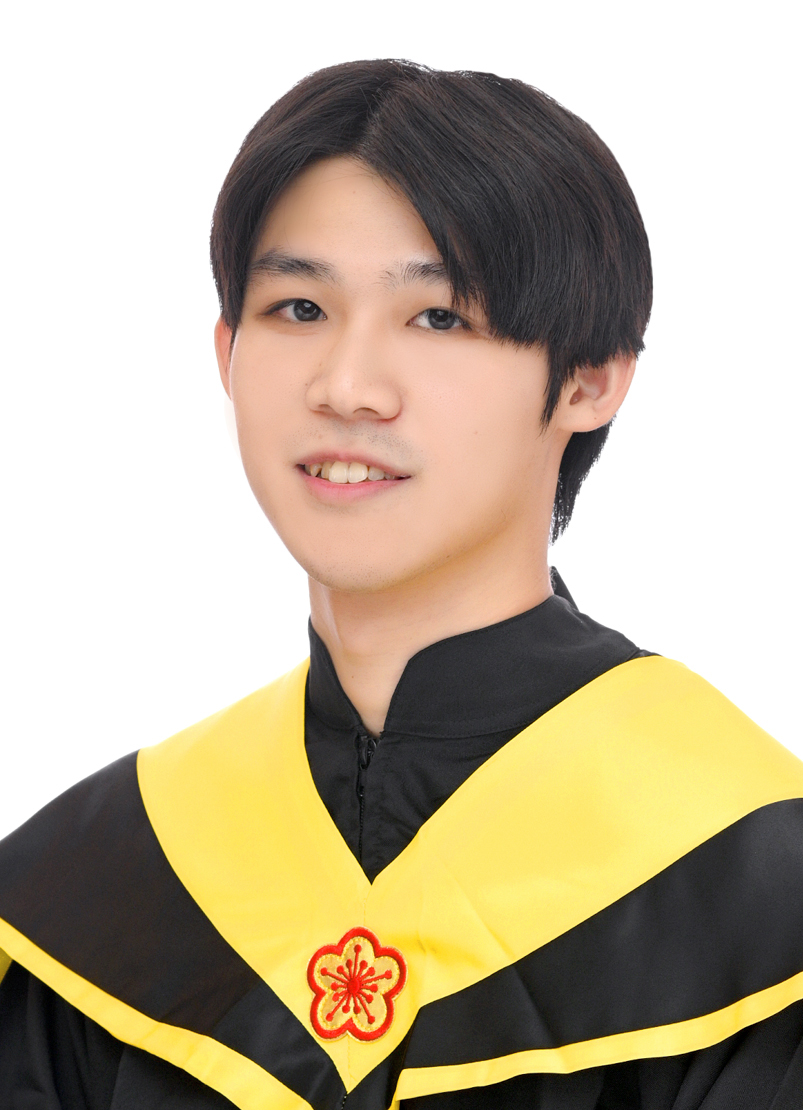
\includegraphics[width=\linewidth, trim=0cm 0.25cm 0cm 0.25cm, clip]{profile/whcheng_profile.jpg} % Add your profile photo here
    \end{minipage}
    \hfill
    \begin{minipage}[t]{0.8\textwidth}
        \begin{header}
            \textbf{\fontsize{24 pt}{24 pt}\selectfont Wei-Hsuan Cheng}

            \vspace{0.3 cm}

            \normalsize

    %%%%%%%%%%%%%%%%%%%%%%%%%%%%%%%%%%
    %%%%%%%%%% Contact info %%%%%%%%%%
    %%%%%%%%%%%%%%%%%%%%%%%%%%%%%%%%%%
        % Location
        \mbox{{\color{black}\footnotesize\faMapMarker*}\hspace*{0.13cm}Taipei, Taiwan}%
        \kern 0.25 cm%
        \AND%
        \kern 0.25 cm%
        % % Email
        % \mbox{\hrefWithoutArrow{mailto:johnathancheng0125@gmail.com}{\color{black}{\footnotesize\faEnvelope[regular]}\hspace*{0.13cm}johnathancheng0125@gmail.com}/\hrefWithoutArrow{mailto:r11631045@ntu.edu.tw}{\color{black}{\footnotesize\faEnvelope[regular]}\hspace*{0.13cm}r11631045@ntu.edu.tw}}%
        % \kern 0.25 cm%
        % \AND%
        % \kern 0.25 cm%
        % Email
        \mbox{\hrefWithoutArrow{mailto:johnathancheng0125@gmail.com}{\color{black}{\footnotesize\faEnvelope[regular]}\hspace*{0.13cm}johnathancheng0125@gmail.com}}%
        \kern 0.25 cm%
        \AND%
        \kern 0.25 cm%
        % TEL
        % \mbox{\hrefWithoutArrow{tel:+90-541-999-99-99}{\color{black}{\footnotesize\faPhone*}\hspace*{0.13cm}0541 999 99 99}}%
        % \kern 0.25 cm%
        % \AND%
        % \kern 0.25 cm%
        % LinkedIn
        \mbox{\hrefWithoutArrow{https://www.linkedin.com/in/wei-hsuan-cheng-582486264/}{\color{black}{\footnotesize\faLinkedinIn}\hspace*{0.13cm}Wei-Hsuan Cheng}}%
        \kern 0.25 cm%
        \AND%
        \kern 0.25 cm%
        % GitHub account
        \mbox{\hrefWithoutArrow{https://github.com/wei-hsuan-cheng}{\color{black}{\footnotesize\faGithub}\hspace*{0.13cm}wei-hsuan-cheng}}%
        \kern 0.25 cm%
        \AND%
        \kern 0.25 cm%
        % Personal website
        \mbox{\hrefWithoutArrow{https://wei-hsuan-cheng.github.io}{\color{black}{\footnotesize\faGlobe}\hspace*{0.13cm}Wei-Hsuan's Homepage}}%
        \end{header}
    \end{minipage}

    \vspace{0.1 cm}


%%%%%%%%%%%%%%%%%%%%%%%%%%%%%%%%%%%%%%%%%
%%%%%%%%%% Research Experience %%%%%%%%%%
%%%%%%%%%%%%%%%%%%%%%%%%%%%%%%%%%%%%%%%%%
    \section{Research Experience}

        \begin{twocolentry}{
        \textit{Taipei, Taiwan}

        \textit{Oct 2025 – Present}}
            \textbf{\href{https://www.deltaww.com/en-US/company/innovation}{Delta Robotics Innovation Center (DRIC)}}

            \textit{Associate Researcher, Delta Electronics, Inc.}
        \end{twocolentry}

        \vspace{0.10 cm}
        \begin{onecolentry}
            \begin{highlights}
                \item Focus on model-based control and estimation methods (e.g., force control, kinematics/dynamics MPC, visual servoing, KF-family).
                \item Develop these methods across various robotic embodiments—including dual-arm systems, dexterous hands, mobile manipulators, and integrated combinations of these platforms, all validated on real hardware.
                \item The dual-arm system, using MPC as whole-body control (WBC) with joint torque sensing for safe physical interaction and 1 kHz EtherCAT communication, was showcased at \textbf{Automation Taipei 2026} (Taipei International Industrial Automation Exhibition).
            \end{highlights}
        \end{onecolentry}

        \vspace{0.2 cm}

        \begin{twocolentry}{
        \textit{Taipei, Taiwan}    
            
        \textit{Dec 2023 – May 2025}}
            \textbf{\href{https://dnc.ntu.edu.tw/en}{Delta-NTU Joint Research \& Development Center}}
            
            \textit{Project lead in the collaboration research project of NTU and the CTO Office in Delta Electronics, Inc.}
        \end{twocolentry}

        \vspace{0.10 cm}
        \begin{onecolentry}
        \needspace{4\baselineskip} % keep this heading with its first bullet
        \textbf{Supervisory Teleoperation of Manipulator for Surveillance}
            \begin{highlights}
                \item Develop a reliable supervisory robotic system for performing dexterous manipulation tasks in industrial surveillance scenario (\textit{e.g.} buttons, switches, and valves operations). The system utilizes a local–remote teleoperation setup with wireless communication, separating the local site—which comprises the control console, user interface, and input device—from the remote site, where the robot performs tasks with sensors and algorithms deployed.
                \item \textbf{Unified 6-DoF Vision Alignment:} Employ a state-of-the-art deep learning method for 6D object pose estimation with a position-based visual servo (PBVS) control scheme. This combination serves as a unified 6-DoF vision alignment method, which is essential for performing precise manipulation tasks for versatile objects in industrial settings.
                \item \textbf{Vision Alignment Corrected by Force:} Apply force control to further correct the vision alignment errors. The integration of two complementary sensory modalities (vision-and-force) provides enhanced accuracy for robotic dexterous manipulation.
            \end{highlights}

The key results of the project were successfully demonstrated to the CEO at the \textbf{2024 Delta
Electronics Annual Innovation Showcase}.


        \end{onecolentry}


        \vspace{0.2 cm}

        \begin{twocolentry}{
        \textit{Taipei, Taiwan}    
            
        \textit{Sept 2022 – May 2025}}
            \textbf{\href{http://rmml.bime.ntu.edu.tw/nturmmle.html}{Robots and Medical Mechatronics Lab (RMML)}}
            
            \textit{Master's student researcher, advised by \hrefWithoutArrow{http://rmml.bime.ntu.edu.tw/profe.html}{Prof. Ping-Lang Yen}}
            
        \end{twocolentry}

        \vspace{0.10 cm}
        \begin{onecolentry}
        \textbf{Project Experiences and Contributions}
            \begin{highlights}
                \item Agricultural Robot:
                \begin{itemize}
                    \item Improve EKF-SLAM for agricultural tracked mobile robot by involving IMU bias estimation and online state covariance update.
                    \item Apply vision-based control scheme and object 6D pose estimation for robotic tomato harvesting.
                \end{itemize}
                \item Surgical Robot:
                \begin{itemize}
                    \item Improve attitude and angular velocity estimation, and the visual servo control scheme for surgical robot end-effector using multi-sensor fusion and a quaternion-based EKF.
                \end{itemize}
            \end{highlights}
        \end{onecolentry}

%%%%%%%%%%%%%%%%%%%%%%%%%%%%%%%
%%%%%%%%%% Education %%%%%%%%%%
%%%%%%%%%%%%%%%%%%%%%%%%%%%%%%%
    \needspace{10\baselineskip} % start Education with its first entry, not one line of it
    \section{Education}
        
        \begin{twocolentry}{
            
            
        \textit{May 2025}}
            \textbf{National Taiwan University (NTU)}

            \textit{Master's in Biomechatronics Engineering}
        \end{twocolentry}

        \vspace{0.10 cm}
        \begin{onecolentry}
            \begin{highlights}
                \item Overall GPA: 4.14/4.3
                \item Scholarships: 2023 Master's Student Scholarship (First Place) from Dept. Biomechatronics Engineering, NTU
                \item \textbf{Coursework:} Robotics, Optimal Control, Stochastic Control, Robust Control, System Identification, Linear Systems
                \item \textbf{Master's Thesis:} Application of Vision- and Force-Based Supervisory Teleoperation for Robotic Dexterous Manipulation Tasks in Industrial Surveillance
            \end{highlights}
        \end{onecolentry}

        \vspace{0.2 cm}

        \begin{twocolentry}{
            
        \textit{June 2022}}
            \textbf{National Tsing Hua University (NTHU)}
            
            \textit{Bachelor in Interdisciplinary Program of Nuclear Science (IPNS)}
        \end{twocolentry}
        \vspace{0.10 cm}
        \begin{onecolentry}
            \begin{highlights}
                \item Specializing in Energy Engineering and Power Mechanical Engineering.
            \end{highlights}
        \end{onecolentry}

%%%%%%%%%%%%%%%%%%%%%%%%%%%%
%%%%%%%%%% Skills %%%%%%%%%%
%%%%%%%%%%%%%%%%%%%%%%%%%%%%
    \section{Skills}

        \begin{onecolentry}
            \textbf{Programming:} C++, Python, MATLAB, JavaScript, LaTeX
        \end{onecolentry}
        \vspace{0.2 cm}
        \begin{onecolentry}
            \textbf{Robotics Research Interests:} Model-based control and estimation for contact-rich/compliant manipulation and legged/wheeled-legged locomotion: Model Predictive Control (MPC), Whole-Body Control (WBC), Kalman Filtering (KF, EKF, UKF, InEKF), Compliance Control (force, admittance, impedance), Vision-based Control, Conformal Geometric Algebra (CGA) in Robotics
        \end{onecolentry}
        \vspace{0.2 cm}
        \begin{onecolentry}
            \textbf{Software/Hardware/Tools:} ROS 1 \& 2, ros2\_control, OCS2, Pinocchio, HPIPM, MuJoCo, JAX, MoveIt 2, BehaviorTree.CPP, PCL, PyQt5, Git, Docker, SolidWorks, Onshape, NVIDIA Jetson, STM32/ESP32 MCU
        \end{onecolentry}

        \vspace{0.2 cm}
        \begin{onecolentry}
            \textbf{Languages:} Mandarin Chinese (native), English (fluent; proficient in academic presentations and team leadership as NTU project lead for a mixed local–international team)
        \end{onecolentry}


%%%%%%%%%%%%%%%%%%%%%%%%%%%%%%%%%%
%%%%%%%%%% Publications %%%%%%%%%%
%%%%%%%%%%%%%%%%%%%%%%%%%%%%%%%%%%
    % \section{Publications}

    %     \begin{samepage}
    %         \begin{twocolentry}{
    %             Jan 2004
    %         }
    %             \textbf{3D Finite Element Analysis of No-Insulation Coils}

    %             \vspace{0.10 cm}

    %             \mbox{Frodo Baggins}, \mbox{\textbf{\textit{Wei-Hsuan Cheng}}}, \mbox{Samwise Gamgee}
    %         \end{twocolentry}


    %         \vspace{0.10 cm}

    %         \begin{onecolentry}
    %     \href{https://doi.org/10.1109/TASC.2023.3340648}{10.1109/TASC.2023.3340648}
    %         \end{onecolentry}
    %     \end{samepage}


%%%%%%%%%%%%%%%%%%%%%%%%%%%%%%%%%%%%%%%
%%%%%%%%%% Selected Projects %%%%%%%%%% 
%%%%%%%%%%%%%%%%%%%%%%%%%%%%%%%%%%%%%%%
    \section{Selected Projects}

        \begin{twocolentry}[4.9 cm]{
        \textit{Nov 2026}
        }
            \textbf{GPU-Accelerated MPC with TurboMPC behind OCS2}
        \end{twocolentry}
        \vspace{0.10 cm}
        \begin{onecolentry}
            \begin{highlights}
                \item Integrate TurboMPC (JAX, CPU or GPU) with FRAX dynamics as the solver behind OCS2 inverse-dynamics MPC controllers in ros2\_control, through a shared-memory Python worker. Validated in MuJoCo simulation.
            \end{highlights}
        \end{onecolentry}
        \vspace{0.2 cm}

        \begin{twocolentry}[4.9 cm]{
        \hrefWithoutArrow{https://github.com/wei-hsuan-cheng/legged_robot_mpc_controller}{{\footnotesize\faGithub}\hspace*{0.13cm}legged\_robot\_mpc\_controller}\\\textit{Oct 2026}
        }
            \textbf{Legged Robot MPC: Whole-Body Inverse-Dynamics MPC for Humanoids and Wheeled-Bipeds}
        \end{twocolentry}
        \vspace{0.10 cm}
        \begin{onecolentry}
            \begin{highlights}
                \item Whole-body inverse-dynamics MPC in ros2\_control for the Unitree G1 and H2 humanoids and the Upkie wheeled biped (OCS2, Pinocchio): optimizes configuration, velocity, contact wrenches, accelerations, and torques over a 1 s horizon under the full rigid-body dynamics, at 100–200 Hz (SQP, HPIPM).
                \item Proprioceptive state estimation without ground truth (contact-aided InEKF or linear KF, as chainable ros2\_control controllers) and a hardware-ready bring-up from a crouch.
                \item Validated in MuJoCo simulation: humanoid walking, running, stumble recovery, and uneven terrain; rolling-contact constraints and a planned stand-up from kneeling for the wheeled biped over ramps and steps.
            \end{highlights}
        \end{onecolentry}
        \vspace{0.2 cm}

        \begin{twocolentry}[4.9 cm]{
        \hrefWithoutArrow{https://github.com/wei-hsuan-cheng/dynamics_mpc_controller}{{\footnotesize\faGithub}\hspace*{0.13cm}dynamics\_mpc\_controller}\\\textit{June 2026}
        }
            \textbf{Robotic Arm Dynamics MPC: Inverse- and Forward-Dynamics MPC}
        \end{twocolentry}
        \vspace{0.10 cm}
        \begin{onecolentry}
            \begin{highlights}
                \item Inverse-dynamics (RNEA equality, optimizing accelerations, torques, and the end-effector wrench) and forward-dynamics (ABA) MPC in ros2\_control for single and dual UR5 arms, built on OCS2 and Pinocchio; real-time-iteration SQP with HPIPM at 100 Hz. Validated in MuJoCo simulation.
                \item Self-collision and moving-obstacle avoidance, with collisions handled by sphere approximation.
                \item External end-effector wrench estimation with a momentum observer.
            \end{highlights}
        \end{onecolentry}
        \vspace{0.2 cm}

        \begin{twocolentry}[4.9 cm]{
        \hrefWithoutArrow{https://github.com/wei-hsuan-cheng/stewart_platform_sim.git}{{\footnotesize\faGithub}\hspace*{0.13cm}stewart\_platform\_sim}\\\textit{July 2025}
        }
            \textbf{stewart\_platform\_sim: Six-DoF Stewart-Gough Platform Simulation}
        \end{twocolentry}
        \vspace{0.10 cm}
        \begin{onecolentry}
            \begin{highlights}
                \item ROS 2 Python simulation of a six-DoF Stewart platform (or Stewart-Gough platform), which is a parallel manipulator comprising a fixed base platform, a moving end-effector platform, and six serial SPS structures.
                \item The inverse kinematics (IK) and differential kinematics (DK) problems are solved to obtain the required leg lengths and leg velocities for driving the robot to achieve a desired motion in $SE(3)$.
            \end{highlights}
        \end{onecolentry}
        \vspace{0.2 cm}

        \begin{twocolentry}[4.9 cm]{
        \hrefWithoutArrow{https://github.com/wei-hsuan-cheng/kendo_robot}{{\footnotesize\faGithub}\hspace*{0.13cm}kendo\_robot}\\\textit{Dec 2023}
        }
            \textbf{Kendo Robot: Combining Robotics Technologies with Martial Art}
        \end{twocolentry}
        \vspace{0.10 cm}
        \begin{onecolentry}
            \begin{highlights}
                \item A supervisory teleoperation kendo robot system. The robotic arm holding kendo sword tracks the opponent’s pose and waits for the operator’s command to attack on different body positions.
                \item Detect and track the 3D human body by DL-based real-time human pose estimation algorithm and RGB-D alignment. An interactive GUI is built using JavaScript for real-time visualization and robotic motion planning.
                \item Robotic arm IK solver and sword motion planner are designed based on a new mathematical framework, conformal geometric algebra (CGA).
                \item Developed using ROS 1 Python, and a web-based interactive GUI using JavaScript. ROS-JavaScript communication through web socket.
            \end{highlights}
        \end{onecolentry}
        \vspace{0.2 cm}

        \begin{twocolentry}[4.9 cm]{
        \hrefWithoutArrow{https://github.com/wei-hsuan-cheng/cga_ik}{{\footnotesize\faGithub}\hspace*{0.13cm}cga\_ik}\\\textit{Nov 2023}
        }
            \textbf{CGA IK: Closed-Form Inverse Kinematics Solver based on CGA}
        \end{twocolentry}
        \vspace{0.10 cm}
        \begin{onecolentry}
            \begin{highlights}
                \item Aim to promote a new mathematical framework \textbf{conformal geometric algebra (CGA)} for robotics applications. 
                \item Implemented closed-form IK solvers for a 6-DoF collaborative robot (cobot) and a 3-DoF spherical parallel manipulator (SPM) based on CGA.
                \item Simulated and visualized in a web-based interactive GUI using JavaScript. Implemented in ROS 2 C++ and tested on a real robot.
            \end{highlights}
        \end{onecolentry}
        \vspace{0.2 cm}

        \begin{twocolentry}[4.9 cm]{
            \hrefWithoutArrow{https://github.com/wei-hsuan-cheng/kf_cpp}{{\footnotesize\faGithub}\hspace*{0.13cm}kf\_cpp}\\\textit{May 2023}
            }

            \textbf{Attitude and Angular Velocity Estimation of Surgical Robot Using Sensor Fusion with Optical Tracker, IMU, and Quaternion-based Extended Kalman Filter}
        \end{twocolentry}
        \vspace{0.10 cm}
        \begin{onecolentry}
            \begin{highlights}
                \item A multi-sensor fusion framework is used for estimating the attitude and angular velocity of surgical robot end-effector, for better robustness (against occlusions) and tracking precision in minimally invasive surgeries.
                \item A quaternion-based EKF algorithm is derived based on a constant angular velocity model.
                \item The EKF and UKF algorithms are implemented in ROS 2 C++.
            \end{highlights}
        \end{onecolentry}

        % \vspace{0.2 cm}

        % \begin{twocolentry}{
        % \textit{Dec 2022}}
        %     \textbf{Furuta Pendulum Balancing Control and Disturbance Rejection via State-Observer Feedback and Internal Model Design}
        % \end{twocolentry}
        % \vspace{0.10 cm}
        % \begin{onecolentry}
        %     \begin{highlights}
        %         \item Stabilize the Furuta pendulum system by the design of state-observer feedback controller. An internal model is utilized to reject the sinusoidal process noise in the input signal of maxon motor. 
        %         \item Course project of EE5128 Linear Systems @ NTU EE. System dynamics and control algorithm are simulated in Simulink, Simscape, and MATLAB.
        %     \end{highlights}
        % \end{onecolentry}
        

%%%%%%%%%%%%%%%%%%%%%%%%%%%%%%%%%%%%%%%%%%%%
%%%%%%%%%% Other Open-Source Work %%%%%%%%%%
%%%%%%%%%%%%%%%%%%%%%%%%%%%%%%%%%%%%%%%%%%%%
    \section{Other Open-Source Work}

        \begin{onecolentry}
            \begin{highlights}
                \item \textbf{\href{https://wei-hsuan-cheng.github.io/robotics-notes/}{Robotics Notes}:} notes documenting my robotics learning journey, from MPC to rigid-body dynamics.
                \item \textbf{Tools:} \mbox{\hrefWithoutArrow{https://github.com/wei-hsuan-cheng/visualize_convex_optimization}{{\footnotesize\faGithub}\hspace*{0.13cm}visualize\_convex\_optimization}} (interactive convex optimization figures), \mbox{\hrefWithoutArrow{https://github.com/wei-hsuan-cheng/m3t_ros2}{{\footnotesize\faGithub}\hspace*{0.13cm}m3t\_ros2}} (M3T object tracking in ROS 2), \mbox{\hrefWithoutArrow{https://github.com/wei-hsuan-cheng/urdf_to_screw_list}{{\footnotesize\faGithub}\hspace*{0.13cm}urdf\_to\_screw\_list}} (URDF to PoE screws).
            \end{highlights}
        \end{onecolentry}

%%%%%%%%%%%%%%%%%%%%%%%%%%%%%%%%%%%%%%%%%
%%%%%%%%%% Teaching Assistants %%%%%%%%%%
%%%%%%%%%%%%%%%%%%%%%%%%%%%%%%%%%%%%%%%%%
    \section{Teaching Assistants (TAs)}
    
        \begin{twocolentry}{
        \textit{Fall 2022}}
            \textbf{Engineering Mathematics (I)}
        \end{twocolentry}

        \vspace{0.2 cm}

        \begin{twocolentry}{
        \textit{Fall 2022}}
            \textbf{Introduction to Foreign Literature on Bio-Systems Engineering}
        \end{twocolentry}
        
%%%%%%%%%%%%%%%%%%%%%%%%%%%%
%%%%%%%%%% Awards %%%%%%%%%%
%%%%%%%%%%%%%%%%%%%%%%%%%%%%
    \section{Awards}
    
        \begin{twocolentry}{
        \textit{Dec 2023}}
            \textbf{Robotics Competition Winner (Kendo Robot)} as team lead in the course project of CSIE5074 Robotics, offered by Prof. Li-Chen Fu @ NTU EE.
        \end{twocolentry}


\end{document}